\chapter{Graph Infection}
\label{graph-infection}
The Graph Infection (GI) algorithm proposed in \cite{konorski2019mitigating} is similar to the SEIRS model, but some changes were made. There are two  healthy states--Susceptible and Quarantine, and two Infected states--Acute and Recoverable. The state transition machine is presented in Fig. \ref{fig:finite-state-machine-jekon}.
\begin{figure}[h!]
    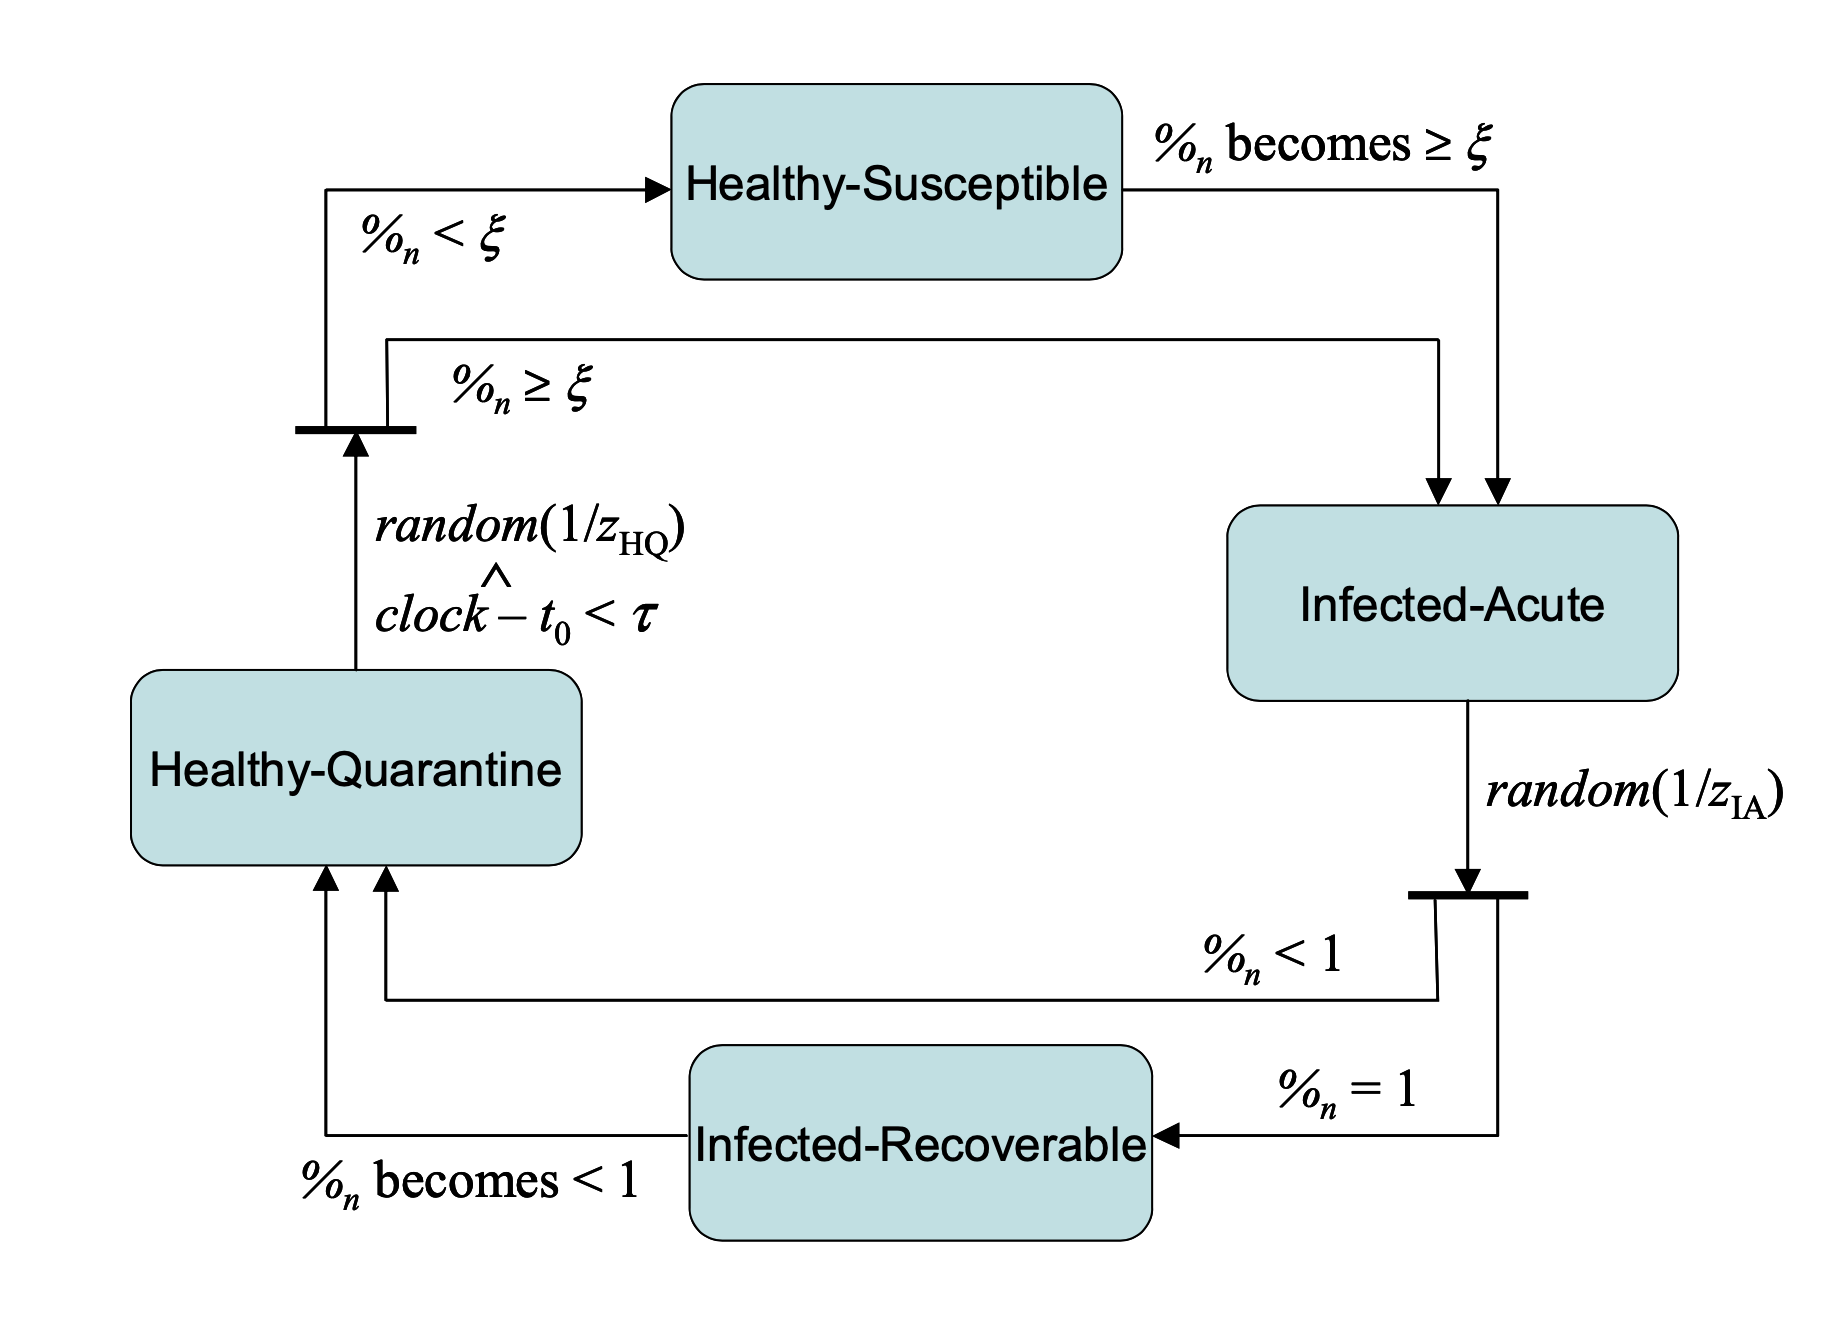
\includegraphics[width=11cm]{img/finite-state-at-node.png}
    \centering
    \caption{Finite state machine at a node. Source: Mitigating Time-Constrained Stolen-Credentials Content Poisoning in an NDN Setting \cite{konorski2019mitigating}}
    \label{fig:finite-state-machine-jekon}
\end{figure} 

The four states can be described as follows:
\begin{itemize}
\item Susceptible nodes are healthy––they do not propagate infection, but can get infected, whereupon change state to Acute.
\item Acute nodes are infected––they inflict infection propagation and switch state to Recoverable or Quarantine depending on how many of their neighbors are infected.
\item Recoverable nodes are infected but can switch to Quarantine if some of their neighbors become healthy.
\item Quarantine nodes are healthy and can switch state to Susceptible or Acute, depending on how many of their neighbors are infected.
\end{itemize}
Nodes can get infected by either:
\begin{enumerate}
    \item external infection -- a content publisher can always infect his/her home node, and then successive nodes at fixed time intervals.
    \item internal infection -- when the fraction of infected neighbors surpasses the $\xi$ threshold. 
\end{enumerate}

Initially, all nodes are healthy (distrust new content). When a publisher wants to authenticate new content, he/she starts the external infection process by infecting his/her assigned home node. The home node imposes a fixed delay, after which it issues a new certificate allowing the publisher to infect the next node selected at random. The publisher infects the next node by presenting the certificate signed by the previous node. This process is repeated until an epidemic occurs or the intruder loses access to the stolen credentials. To give this process some momentum, we allow the infected nodes to infect others in a process of internal infections. In this way, the publisher does not need to coordinate the whole process until the network reaches epidemic, but just starts a "chain reaction", and if he/she does so with sufficient power, an epidemic will occur.

Internal infections work as follows: a node $n$ in the Susceptible state switches to the Acute state by being infected by a sufficient proportion of its neighbors, specifically if the fraction of its infected neighbors $\%_n = \frac{|I_n|}{|N_n|}$ reaches the threshold $\xi$, where $I_n$ is the set of infected $n$'s neighbors and $N_n$ is the set of all $n$'s neighbors. For simplicity let us measure time in units called \textit{cycles}, a cycle being long enough for a node to infect a neighbor node. To give the process some momentum, the Acute and Quarantine states are introduced. A node has to spend some random time before leaving either state, denoted $random(\frac{1}{Z_{IA}})$ and $random(\frac{1}{Z_{HQ}})$, respectively, where $Z_{IA}$ is the mean number of cycles in the Acute state, and $Z_{HQ}$ is the mean number of cycles in the Quarantine state. Depending on $\%_n$, a node leaving the Acute state switches either to Recoverable––if $\%_n = 1$, or directly to Quarantine––if $\%_n < 1$. In the Recoverable state, the node is still infected, but as soon as one of its neighbors recovers, it switches to the Quarantine state. The Quarantine state is similar to Acute except that a node can be locked in this state forever if it gets immunized. The immunization is acquired after $\tau$ cycles from the first infection on the node, where $\tau$ is a fixed parameter working as a timeout, preventing an endemic (partial epidemic) of the network. If an endemic were to prevail for a long time, it would mean that the publisher's proof-of-time was too weak to reach an epidemic, but too strong for all the nodes to recover.

As we discussed earlier, there is no known analytical solution to such a graph model; therefore, it needs to be computer simulated.

\section{Simulator}
\label{simulator}
\begin{figure}[h!]
  \subfloat[Visual simulator]{
	\begin{minipage}[c][1\width]{
	   0.5\textwidth}
	   \centering
	   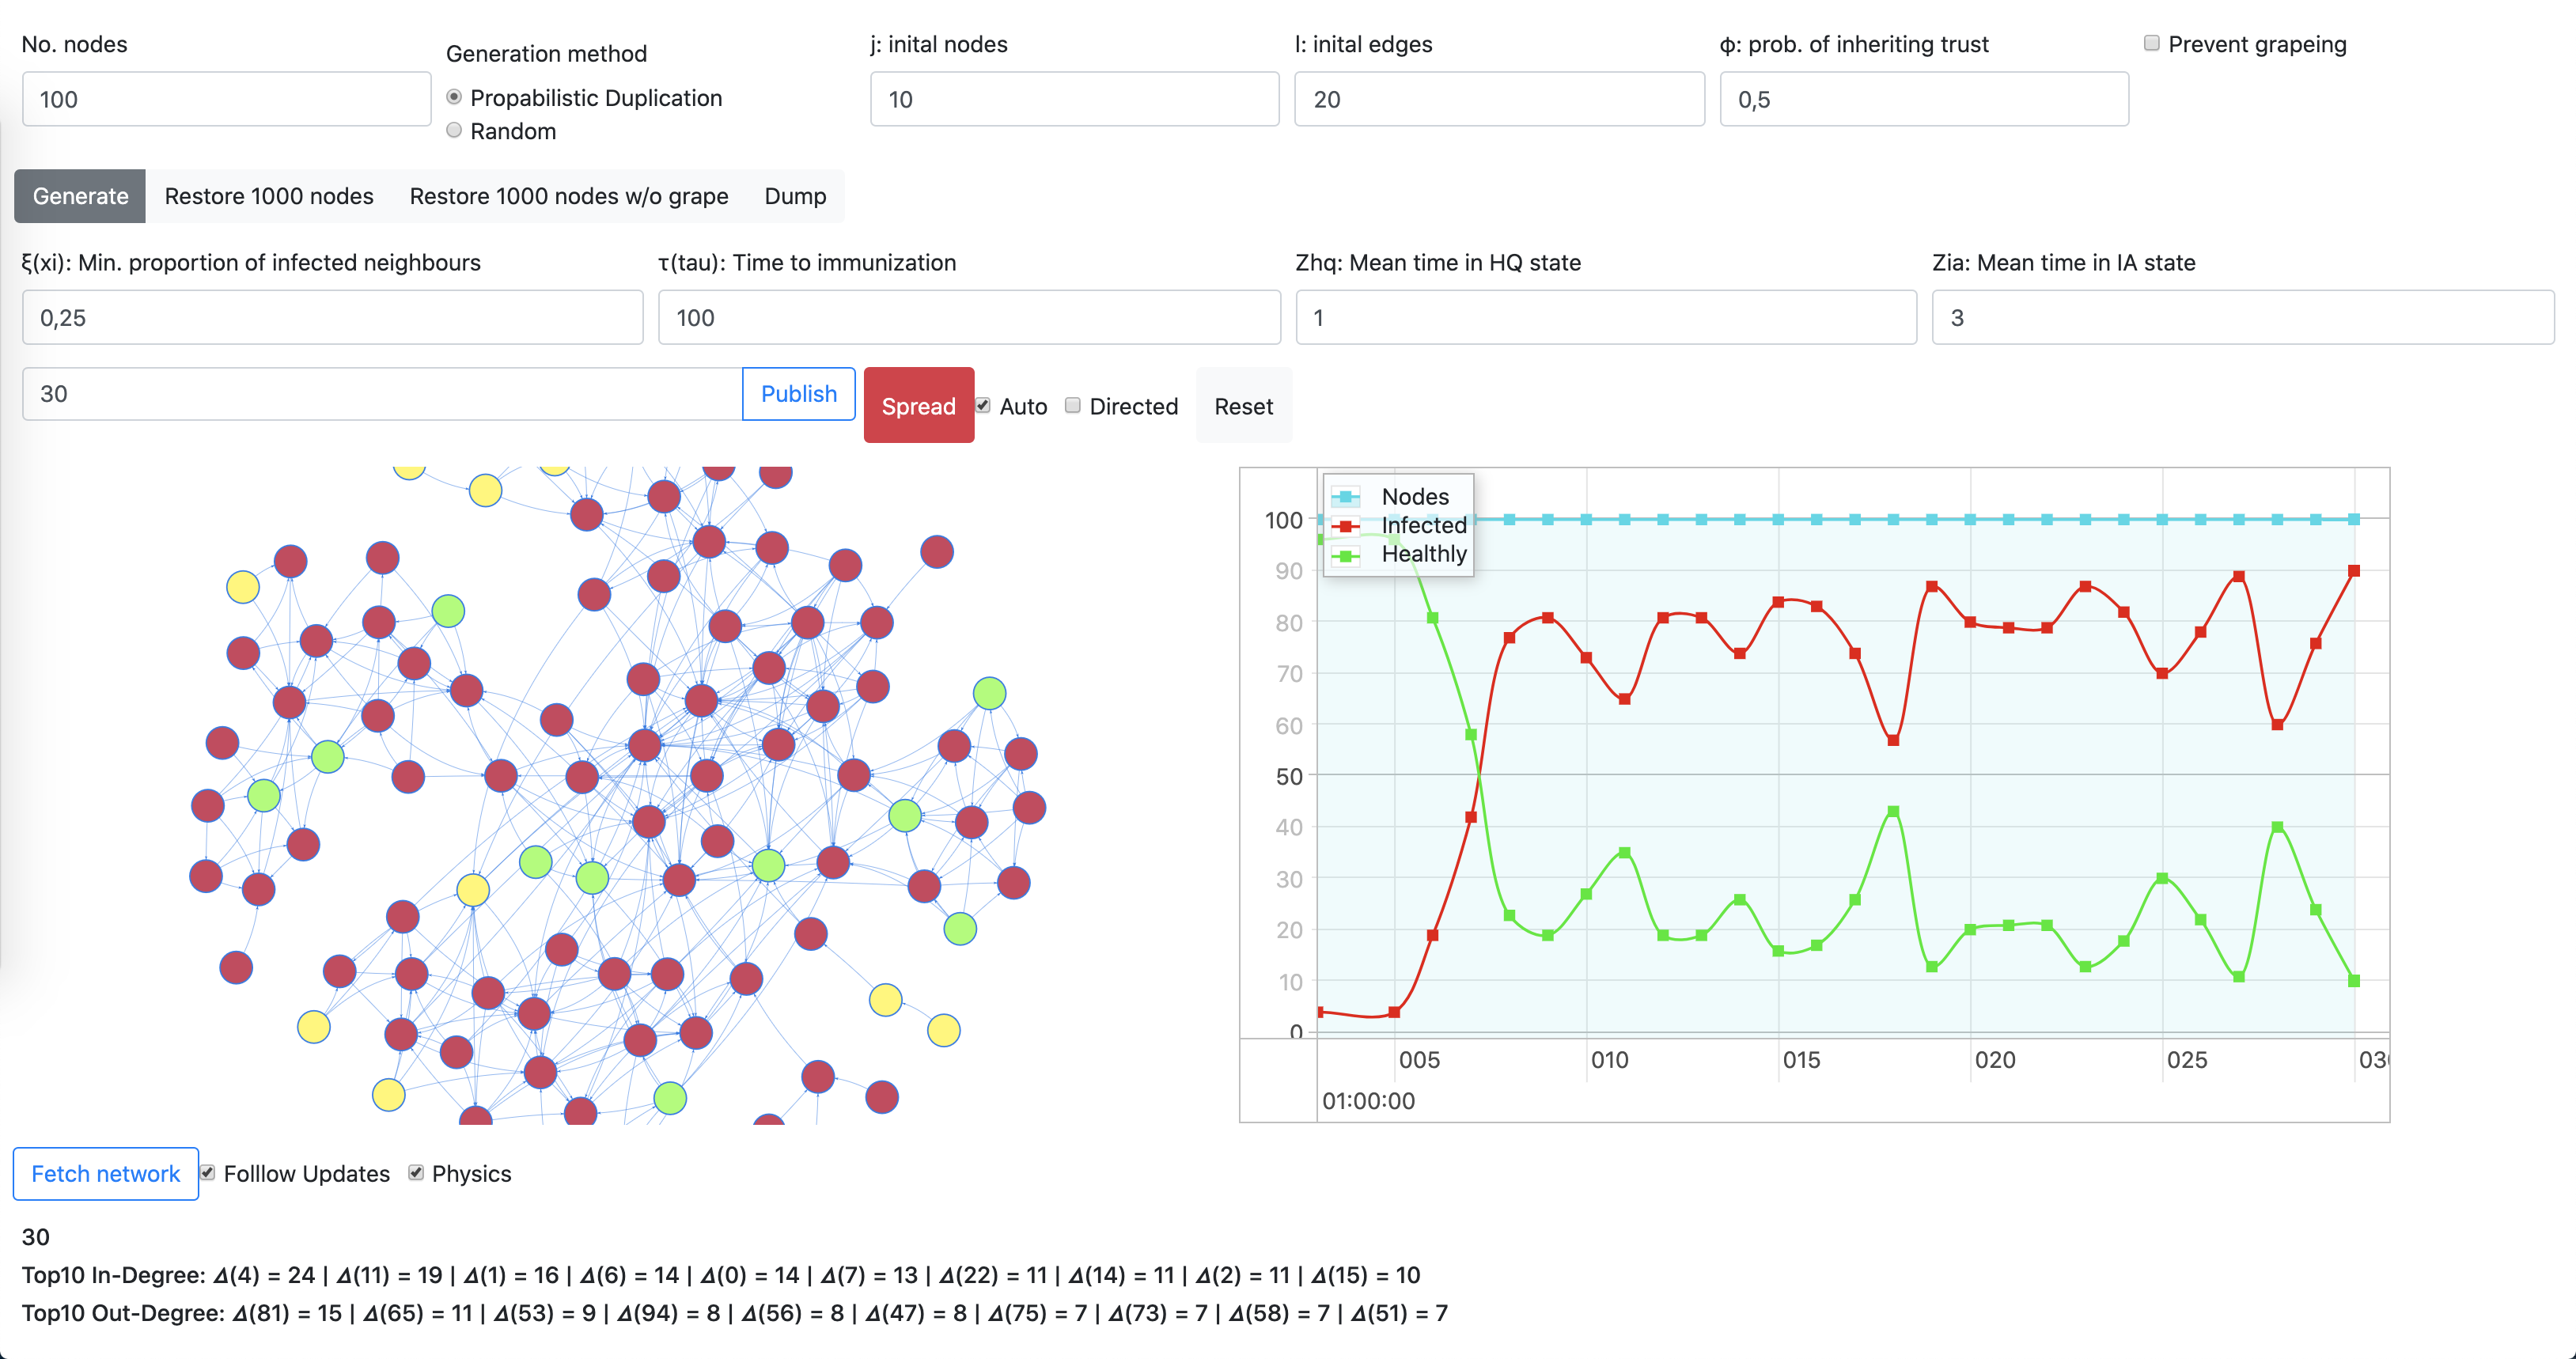
\includegraphics[width=1\textwidth]{img/simulator.png}
	\end{minipage}}
 \hfill 	
  \subfloat[Fast simulator]{
	\begin{minipage}[c][1\width]{
	   0.5\textwidth}
	   \centering
	   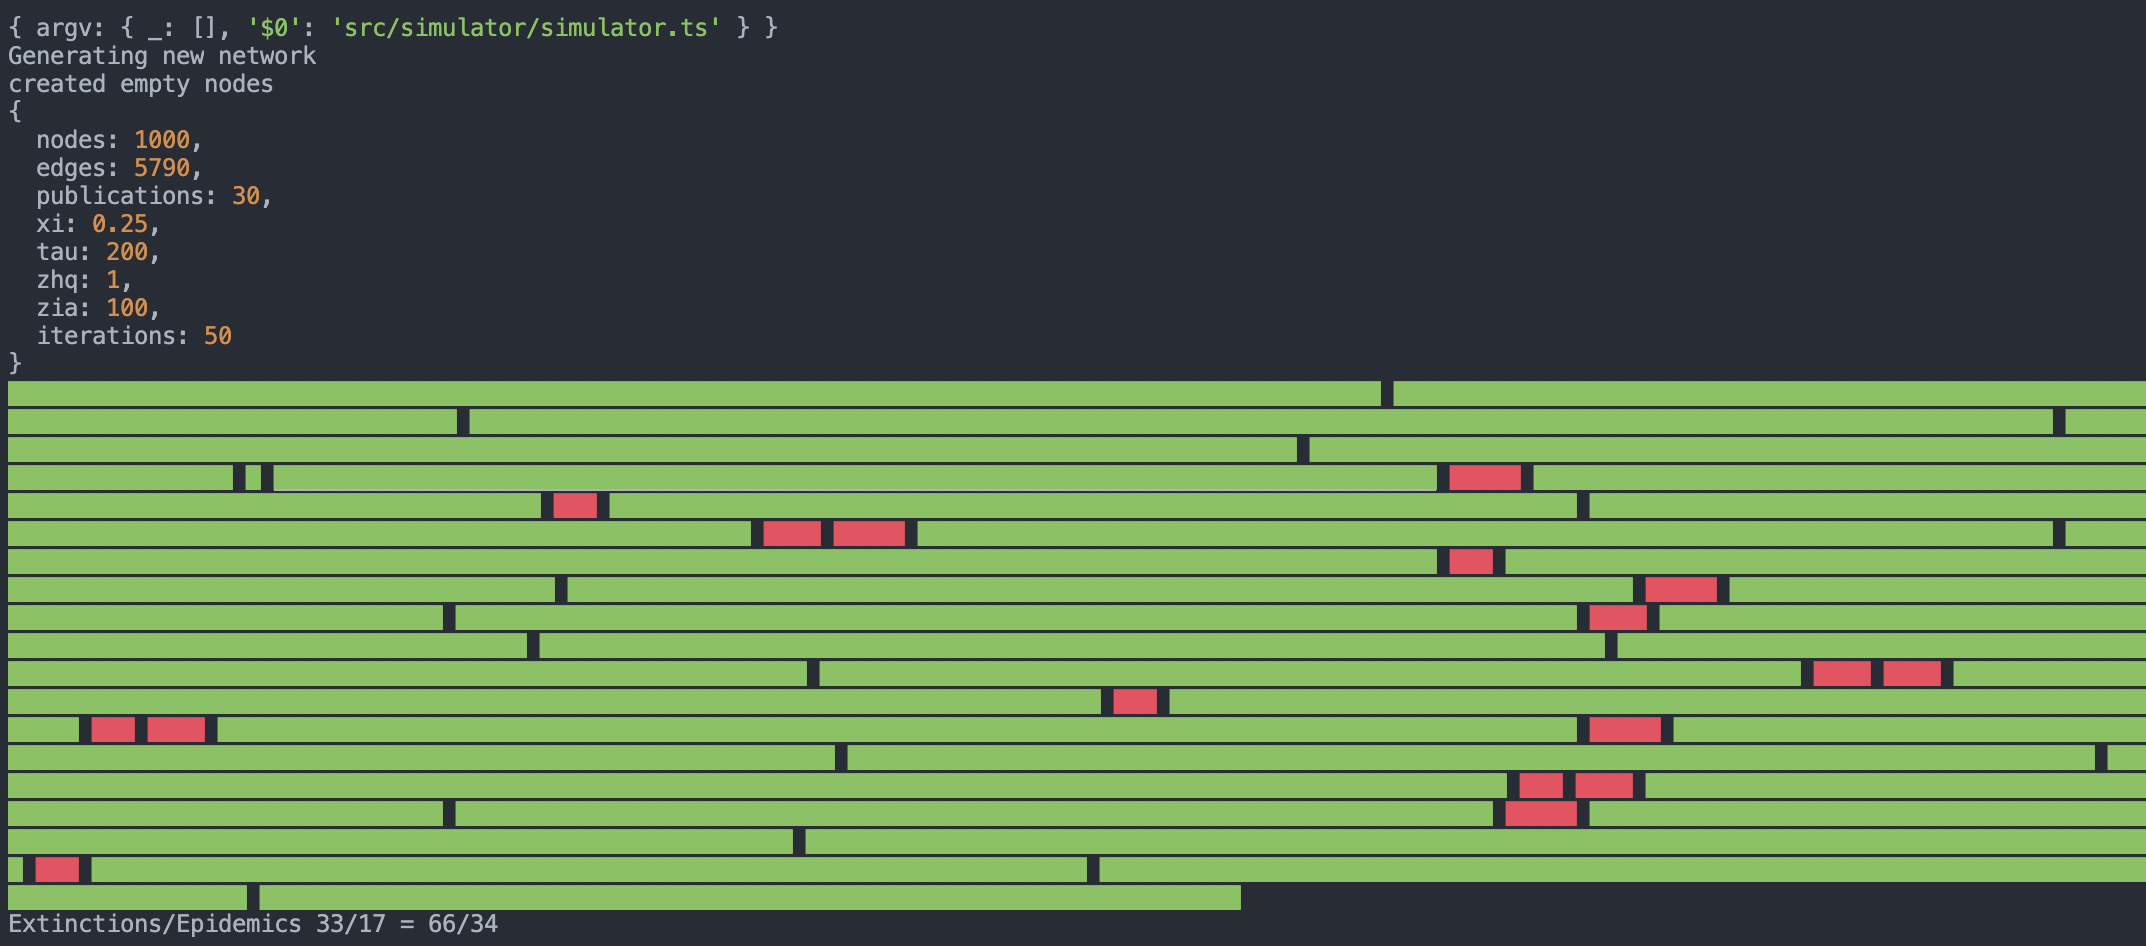
\includegraphics[width=1.1\textwidth]{img/fastsimulator.png}
	\end{minipage}}
\caption{Simulators preview}
\label{fig:simulators}
\end{figure}
We have developed two simulators, the first for visualization and the second for fast calculations. The visualization simulator helps to better understand the processes on graphs and find potential problems. The fast simulator allows to perform various calculations on different input data in a reasonable time. The source code for both simulators is available at \url{https://github.com/stasbar/ProofOfTime-Auth}. Both simulators are presented in Fig. \ref{fig:simulators}. The visual simulator is accessible at \url{masti.stasbar.com}.
Both simulators allow us to generate the trust graph using three different generators: random, web of trust, and probabilistic duplication discussed in Chapter \ref{trust-graph} with customized parameters: number of nodes, number of nodes and edges in the initial kernel, and $\phi$, used in the web of trust and probabilistic duplication to customize the density of the connections. After the graph is generated, one can save and restore it to always work on the same graph during further research. 
When the graph is loaded, we can configure the parameters $\xi$, $\tau$, $Z_{HQ}$, $Z_{IA}$ and the number of external infections (i.e., publications or proofs-of-time).
The fast simulator outputs the results of simulations; the green color indicates that the network ended up in an extinction (all nodes have recovered) and the red color indicates an epidemic; the length of the block indicates the number of cycles needed to reach one of these outcomes. The visual simulator provides a live preview of the graph and a chart of the ongoing infection process.  


\section{Observations}
\label{observations}

We run the simulator against many different configurations to find the influence of each parameter. The algorithm's probabilistic nature forces us to run the simulation multiple (in our case, 200) times for each configuration to get credible results. We run the simulation on 1000-node graphs generated using both web of trust (WoT), random(RND), and probabilistic duplication (PD) generators, but for each simulation, we use the same generated graph. First we investigate the $Z_{IA}$ parameter by assuming all remaining parameters constant: $\xi=0.25, Z_{HQ} = 1, \tau=200$ with the maximum number of external infections (publications) equal to 300.
\begin{figure}[h!]
    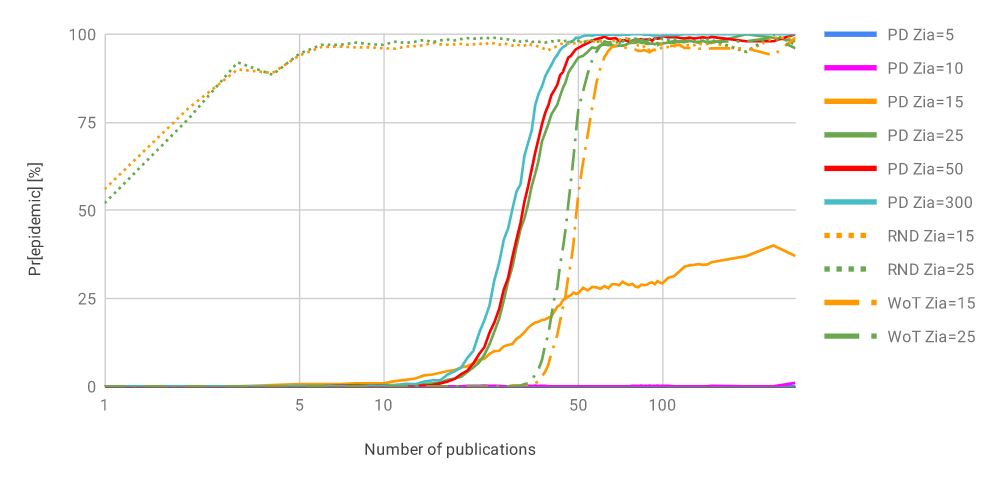
\includegraphics[width=\textwidth]{img/influence-of-zia.png}
    \centering
    \caption{Influence of $Z_{IA}$ parameter}
    \label{fig:influence-of-zia}
\end{figure} 
Figure \ref{fig:influence-of-zia} shows how $Z_{IA}$ influences the probability of reaching an epidemic, (Pr[epidemic]), against the number of external publications (proof-of-time). It does not come as a surprise that the higher $Z_{IA}$, the longer nodes stay infected, and the faster an epidemic is reached. The PD and WoT graphs produce similar shapes. The WoT graph starts to reach an epidemic a little later. 
The RND graph is completely different; even with a low $Z_{IA}$, it reaches an epidemic with just one publication. It happens because most of the nodes have only one or two edges. As a result, one infected node can infect most of its neighbors. In contrast, the PD and WoT graphs often produce nodes of a high degree that are hardly infected by their neighbors.
For all graphs with $Z_{IA}$ starting from 25, the chance of reaching an epidemic in near 100\% starts at about 50-80 external publications. E.g., if we assume the required proof-of-time amounts to 12h, the publisher needs to publish the proof-of-time each 9 to 14 minutes until an epidemic becomes certain.

\begin{figure}[h!]
    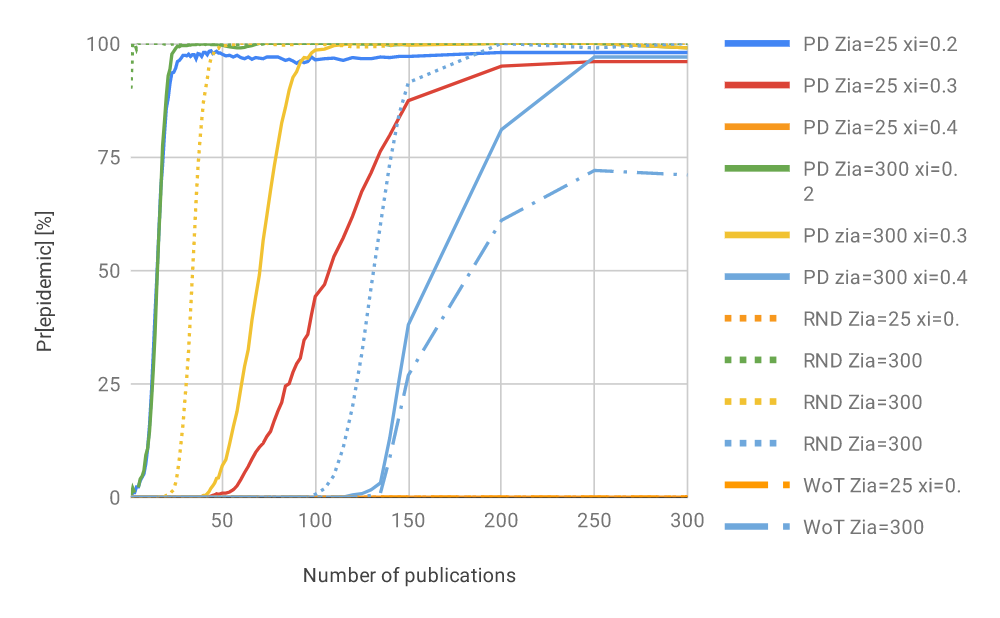
\includegraphics[width=\textwidth]{img/influence-of-xi.png}
    \centering
    \caption{Influence of $\xi$ parameter}
    \label{fig:influence-of-xi}
\end{figure} 
In a similar way, we test the $\xi$ value. Figure \ref{fig:influence-of-xi} shows the Pr[epidemics] against the proof-of-time using different $\xi$ values. We can easily see that $\xi$ is the most sensitive parameter. For values starting from $\xi=0.5$ not a single epidemic simulation occured for any graph generator.

\begin{figure}[h!]
    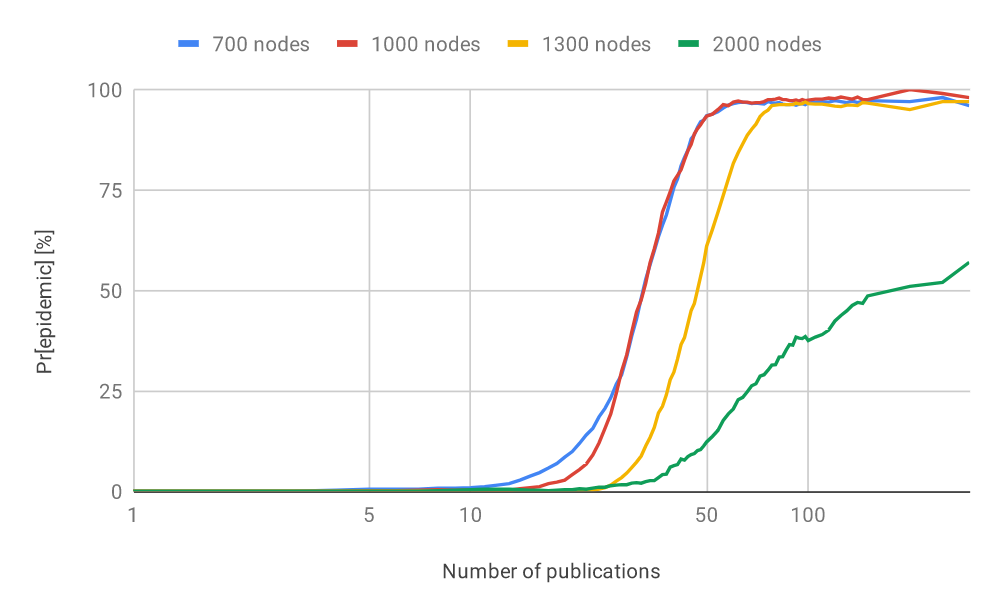
\includegraphics[width=\textwidth]{img/Influence-of-network-size.png}
    \centering
    \caption{Influence of network size}
    \label{fig:influence-network-size}
\end{figure} 
We notice that the parameters $Z_{ia}$ and $xi$ can completely change the outcome depending on the graph type. Their universal values may be hard to find if we want a solution that works on all types of trust networks. Moreover, if we want to set a fixed number of external publications needed to achieve an epidemic, those values should be dynamically changed according to the size of the network.
For example for $\xi=0.25$, $Z_{IA}=25$, $Z_{HQ}=1$, $\tau=200$ the probability of epidemic is significantly influenced by the size of the graph (see Figure \ref{fig:influence-network-size}). Therefore we believe that those parameters should be dynamically adjusted with the network structure changes.

\begin{figure}[h!]
    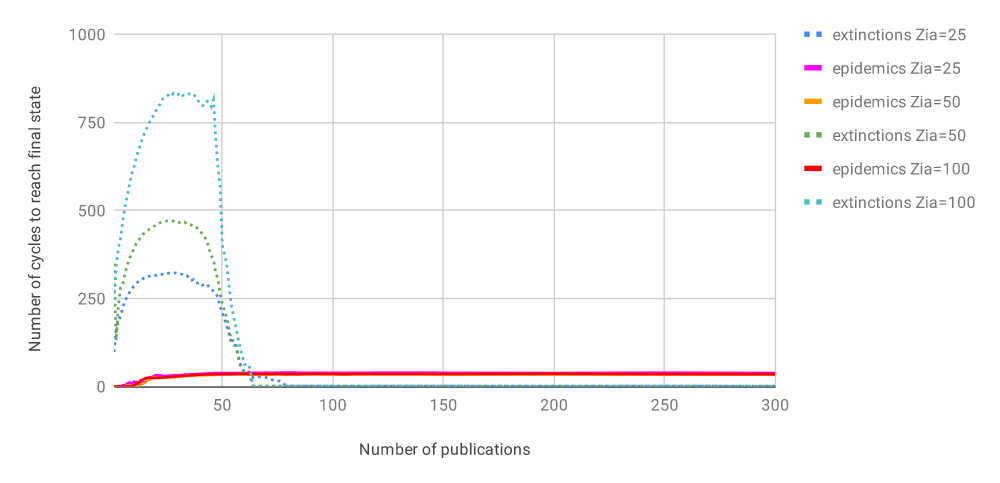
\includegraphics[width=\textwidth]{img/average-number-of-cycles-to-reach-final-state.png}
    \centering
    \caption{Average number of cycles to reach a final outcome}
    \label{fig:average-number-of-cycles}
\end{figure}
An interesting observation relates to the average number of cycles the simulation needs to finish at some final outcome given $Z_{IA}$ (see Figure \ref{fig:average-number-of-cycles}). The average number of cycles needed to reach an extinction grows rapidly until the probability of an extinction is greater than the probability of an epidemic. (Intuitively, the equilibrium point at which the network has the same chance to reach an extinction and an epidemic corresponds to the longest a simulation run can get.) A growing $Z_{IA}$ first increases this number by keeping the nodes in the infected state for a higher number of cycles, then decreases it to zero––indicating that the network can not reach an extinction anymore, or when it does, it reaches it quickly.
The average number of cycles to reach an epidemic is stable at 33 to 38 cycles, perfectly matching the average number of publications needed to reach an epidemic. Intuition tells us that if the network has not reached an epidemic by the time of the last publication (or few cycles after it), there is no chance of reaching an epidemic--the number of external infections was too small.

Another thing that looks strange is that even with many publications, there still exist simulations where the network does not reach an epidemic. To find an explanation of this riddle, we run visual simulation hoping for a clue. This provides us some interesting feedback--some "unfortunate" graph instances and $\xi$ values prevent the whole network from reaching an epidemic even with a large number of external infections (proofs-of-time).
If in a trust graph there exists a \textit{defensive alliance} $A \subseteq N$ of connected nodes where each node $v \in A$ is connected to fewer than $\xi * |N(v)|$ nodes outside $A$, then such an alliance prevents than epidemic. If we assume $\xi = \frac{1}{4}$ and the graph structure visible in \ref{fig:defensive-alliance}a,
\begin{figure}[h!]
  \subfloat[]{
	\begin{minipage}[c][1\width]{
	   0.5\textwidth}
	   \centering
	   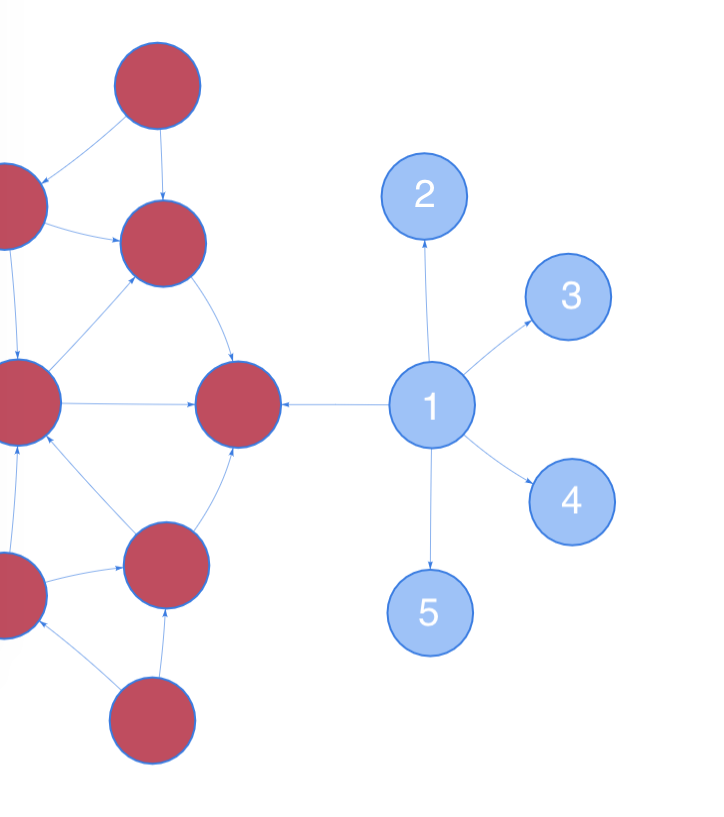
\includegraphics[height=1.0\textwidth]{img/offensive-alliance-numbered.png}
	\end{minipage}}
 \hfill 	
  \subfloat[]{
	\begin{minipage}[c][1\width]{
	   0.5\textwidth}
	   \centering
	   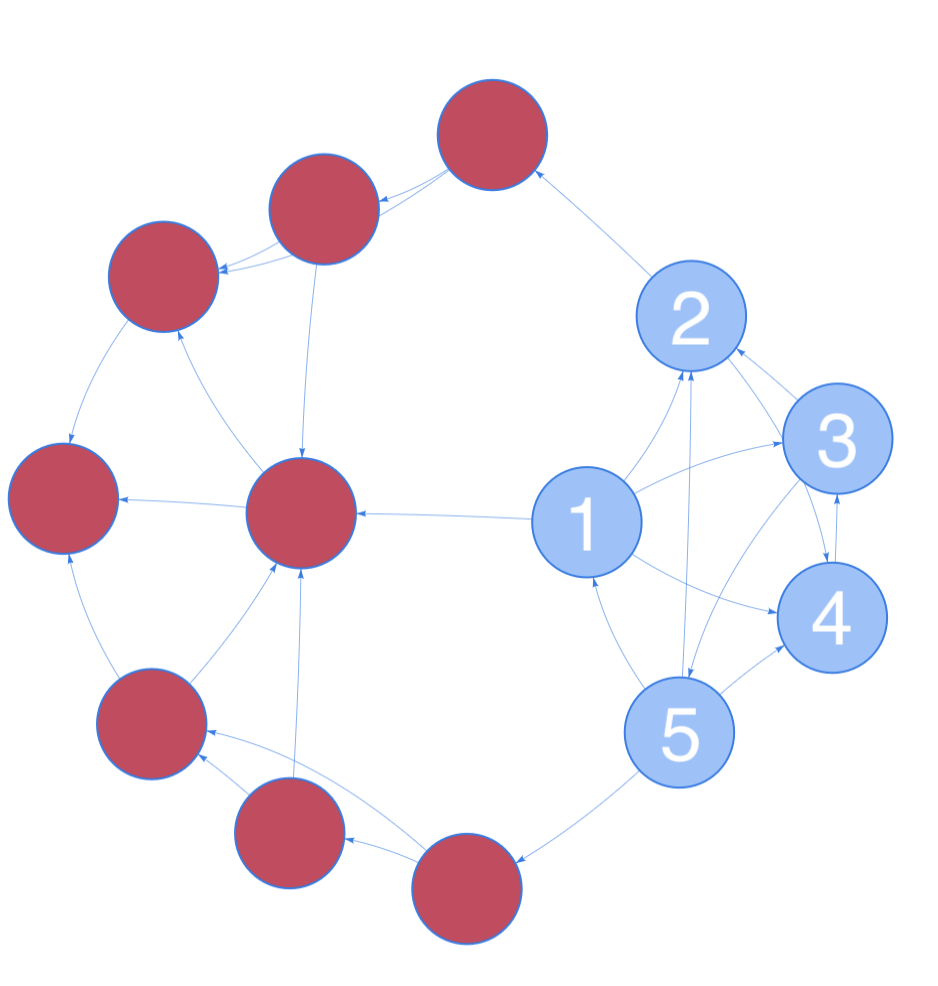
\includegraphics[height=1.0\textwidth]{img/offensive-alliance-clique-numbered.png}
	\end{minipage}}
\caption{Defensive Alliance}
\label{fig:defensive-alliance}
\end{figure}
then the infected nodes (in red) are not able to infect the healthy ones (in blue), especially $v_1$, which is the single node connected to the outside of $A$. It happens because the healthy node $v_1$ has five neighbor nodes, of which four are healthy ($\{v_2,v_3,v_4,v_5\}$), hence the one infected neighbor node is not enough to reach the $\xi = \frac{1}{4}$ threshold at $v_1$.
Let us take a different graph where defensive alliance $A$ is connected to rest of the graph $N \setminus A$ through more than one node as shown in \ref{fig:defensive-alliance}b. Nodes from $A$ cannot be infected since there are not enough connections from outside $A$ to reach the $\xi$ threshold. A general defensive alliance is defined by: 
\begin{equation}
\forall{v \in A}, \frac{|N(v) \cap A|}{|N(v)|} > 1 - \xi.
\end{equation}
As a result, the rest of the network stays in the Acute state until the nodes connected to $A$ change their state to Quarantine (notice that their $\%_n$ are less than 1), which then propagates throughout the rest of the network leading to an extinction. 

To eliminate defensive alliances, we could modify the trust graph generator, but that would violate our assumption that the structure of the trust is taken as a given. Lowering $\xi$ might be another option, but in this way, we would speed up the infection process on the whole network, which is an unwanted effect.

The problem of finding a defensive alliance is NP-complete \cite{ouazine2018alliances}. There is no known solution to finding defensive alliances or even answering in polynomial time whether there exists one in the graph. Therefore the only way of locating defensive alliances in the graph is an exhaustive search. The problem gets even worse if we assume that the network is open, i.e., at any moment nodes can join or leave. 